\chapter{User Guide}
\label{chap:appendix-e}
This guide will cover how to use the solution from a day two perspective after the solution has been integrated with the ACI fabric and vCenter environment.
The rackspace page is the main page of the solution, this page will show the rackspace that is currently available and in use by projects. Additional racks can be deployed by dragging a rack node from the bottom left of the screen. A label can also be dragged onto the floorplan to store text that may be deemed useful. A rack can then be assigned a \gls{tor} node (either a leaf or a FEX) and a terminal server, this should represent what hardware is physically deployed in the rack to ensure the correct connectivity is deployed to the racks.

A project can then be deployed via the projects page, where all information required by the platform is requested via the form. The racks that the project should occupy can be selected via shift-clicking on the racks to select multiple. In the infrastructure tab, the Project Subnet section is the network that will be used internally by the testbed network, if left blank, then the automation platform will automatically assign a non-overlapping subnet to the project. If a specific subnet is required, then this can be specified. The virtual router will be provisioned to the last available IP address in the subnet, and the terminal servers will be assigned sequential addresses starting from the first available IP address in the subnet. The WAN address for the project is also provided, these addresses will be automatically pushed to the virtual router to provide internet connectivity to the project. This form is shown for reference below.

\begin{figure}[H]
    \centering
    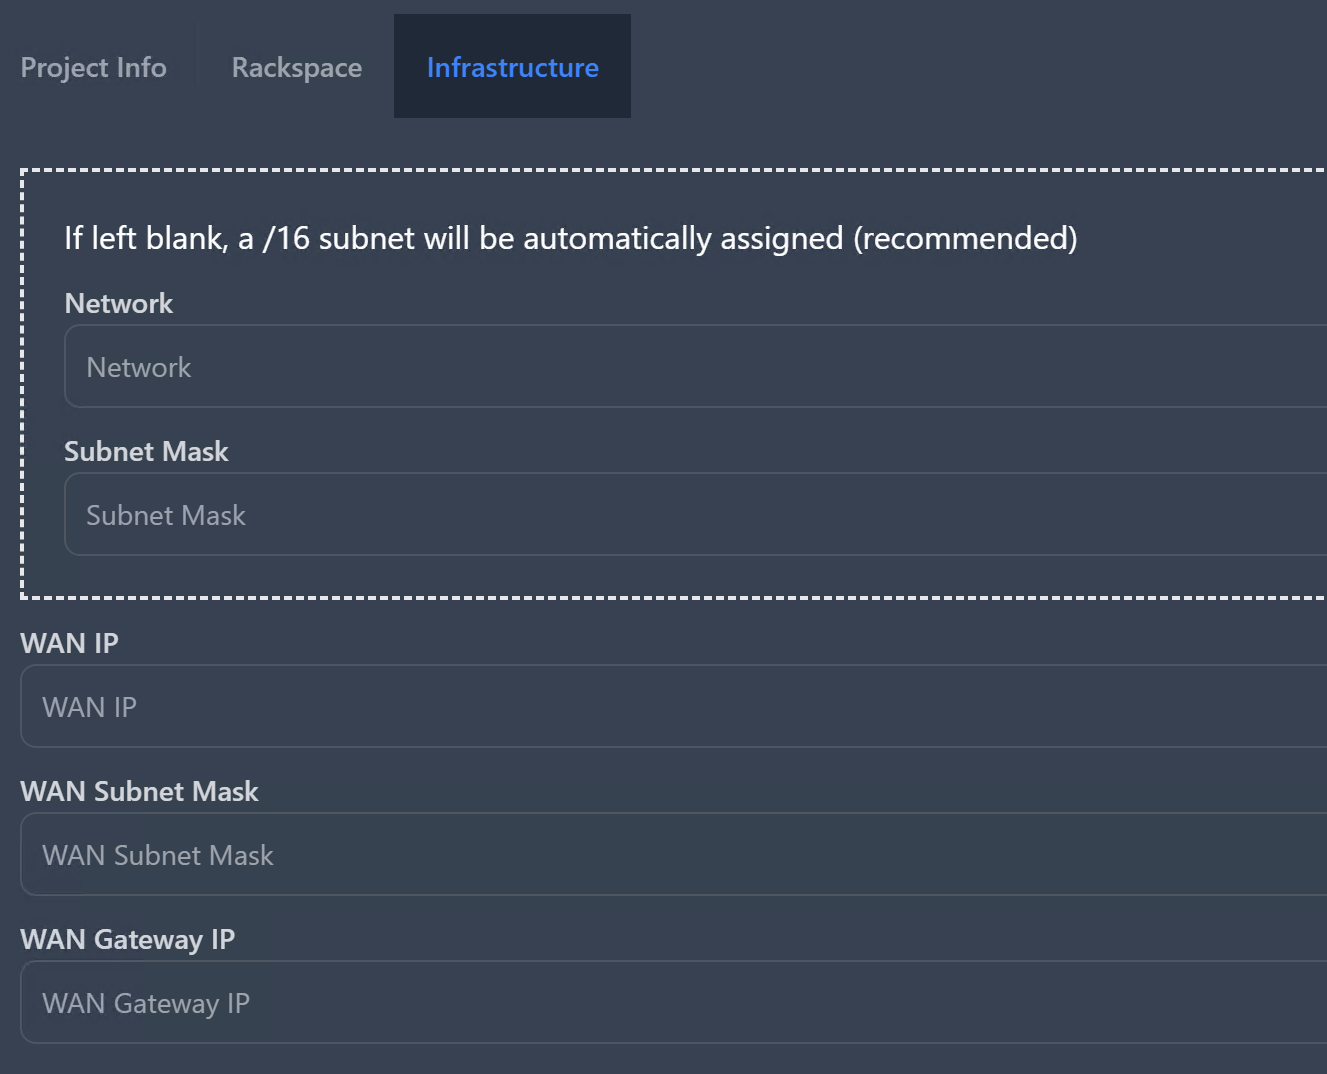
\includegraphics[width=0.8\linewidth]{images/add-project-infrastructure.png}
    \caption{Project Creation Form - Infrastructure}
    \label{fig:userguide1}
\end{figure}

When the project is deployed, the status of the project will update as the deployment progresses through the ACI and VMware deployment phases. Once deployed, a project can then be edited, to modify its occupation of the rackspace. Racks can either be added or removed to a project, allowing its consumption of rackspace to change throughout the lifecycle of the project. Some aspects, such as the name and IP address cannot be changed, and a project must be deleted and recreated if these need to be changed.